%%%%%%%%%%%%%%%%%%%%%%%%%%%%%%%%%%%%%%%%%
% Beamer Presentation
% LaTeX Template
% Version 1.0 (10/11/12)
%
% This template has been downloaded from:
% http://www.LaTeXTemplates.com
%
% License:
% CC BY-NC-SA 3.0 (http://creativecommons.org/licenses/by-nc-sa/3.0/)
%
%%%%%%%%%%%%%%%%%%%%%%%%%%%%%%%%%%%%%%%%%

%----------------------------------------------------------------------------------------
%	PACKAGES AND THEMES
%----------------------------------------------------------------------------------------
\documentclass{beamer}
\usepackage[utf8]{inputenc}
\mode<presentation> {

% The Beamer class comes with a number of default slide themes
% which change the colors and layouts of slides. Below this is a list
% of all the themes, uncomment each in turn to see what they look like.

%\usetheme{default}
%\usetheme{AnnArbor}
%\usetheme{Antibes}
%\usetheme{Bergen}
%\usetheme{Berkeley}
%\usetheme{Berlin}
%\usetheme{Boadilla}
%\usetheme{CambridgeUS}
%\usetheme{Copenhagen}
%\usetheme{Darmstadt}
%\usetheme{Dresden}
%\usetheme{Frankfurt}
%\usetheme{Goettingen}
%\usetheme{Hannover}
%\usetheme{Ilmenau}
%\usetheme{JuanLesPins}
%\usetheme{Luebeck}
\usetheme{Madrid}
%\usetheme{Malmoe}
%\usetheme{Marburg}
%\usetheme{Montpellier}
%\usetheme{PaloAlto}
%\usetheme{Pittsburgh}
%\usetheme{Rochester}
%\usetheme{Singapore}
%\usetheme{Szeged}
%\usetheme{Warsaw}

% As well as themes, the Beamer class has a number of color themes
% for any slide theme. Uncomment each of these in turn to see how it
% changes the colors of your current slide theme.

%\usecolortheme{albatross}
%\usecolortheme{beaver}
%\usecolortheme{beetle}
%\usecolortheme{crane}
%\usecolortheme{dolphin}
%\usecolortheme{dove}
%\usecolortheme{fly}
%\usecolortheme{lily}
%\usecolortheme{orchid}
%\usecolortheme{rose}
%\usecolortheme{seagull}
%\usecolortheme{seahorse}
%\usecolortheme{whale}
%\usecolortheme{wolverine}

%\setbeamertemplate{footline} % To remove the footer line in all slides uncomment this line
%\setbeamertemplate{footline}[page number] % To replace the footer line in all slides with a simple slide count uncomment this line

%\setbeamertemplate{navigation symbols}{} % To remove the navigation symbols from the bottom of all slides uncomment this line
}

\usepackage{graphicx} % Allows including images
\usepackage{booktabs} % Allows the use of \toprule, \midrule and \bottomrule in tables

%----------------------------------------------------------------------------------------
%	TITLE PAGE
%----------------------------------------------------------------------------------------

\title[Transformada de Hough Generalizada]{Transformada de Hough Generalizada} % The short title appears at the bottom of every slide, the full title is only on the title page

\author{Tomás Cerdá, Marcelo Lynch} % Your name
\institute[ITBA] % Your institution as it will appear on the bottom of every slide, may be shorthand to save space
{
Análisis y Tratamiento de Imágenes \\
Instituto Tecnológico de Buenos Aires \\ % Your institution for the title page
\medskip
}
\date{\today} % Date, can be changed to a custom date

\begin{document}

\begin{frame}
\titlepage % Print the title page as the first slide
\end{frame}

\begin{frame}
\frametitle{Contenidos} % Table of contents slide, comment this block out to remove it
\tableofcontents % Throughout your presentation, if you choose to use \section{} and \subsection{} commands, these will automatically be printed on this slide as an overview of your presentation
\end{frame}

%----------------------------------------------------------------------------------------
%	PRESENTATION SLIDES
%----------------------------------------------------------------------------------------

%------------------------------------------------
\section{Transformada clásica de Hough} % Sections can be created in order to organize your presentation into discrete blocks, all sections and subsections are automatically printed in the table of contents as an overview of the talk
%------------------------------------------------

\subsection{Características} % A subsection can be created just before a set of slides with a common theme to further break down your presentation into chunks

\begin{frame}
\frametitle{Transformada clásica}
\begin{itemize}
\item Nos permite encontrar curvas solo si están dadas por ecuaciones paramétricas $f(\textbf{x},\textbf{a}) = 0$
\item Costo computacional elevado: ante $m$ parámetros con $M$ valores posibles y con $p$ píxeles de borde en la imagen
  \begin{itemize}
     \item Algoritmo general / naïve: $O(pM^m)$
     \item Un parámetro puede determinarse de la ecuación $f(\textbf{x},\textbf{a}) = 0$, volviéndolo $O(pM^{m-1})$
     \item Puede reducirse usando información direccional a $O(pM^{m-2})$
   \end{itemize}
\end{itemize}
\end{frame}

%------------------------------------------------
\subsection{El algoritmo más general} % A subsection can be created just before a set of slides with a common theme to further break down your presentation into chunks

\begin{frame}
\frametitle{Algoritmo general}
\begin{enumerate}
    \item Inicializar un arreglo de votación $A(\textbf{a})$
    \item Para cada píxel de borde $\textbf{x}$ y para cada $\textbf{a}$ en el espacio de parametros discretizado, si $f(\textbf{x},\textbf{a}) < \epsilon$, hacer $A(\textbf{a}) = A(\textbf{a})+1$
    \item Buscar máximos locales en $A$, que determinan los parámetros de las curvas presentes en la imagen 
\end{enumerate}

Recorro todo el espacio de parámetros para cada pixel de borde: $O(pM^m)$.
\end{frame}
\begin{frame}{Información extra}
Si se están buscando curvas dadas por una ecuación específica, podemos utilizarla para reducir la exploración del espacio de parámetros.
\\
Ejemplo: supongamos que queremos detectar elipses. Tenemos:
\begin{align*}
    \frac{x - x_0}{a^2} + \frac{y - y_0}{b^2} = 1
\end{align*}
Los parámetros son $x_0, y_0, a, b$.
\end{frame}
\subsection{Mejorando el algoritmo en casos particulares}
\begin{frame}{Utilizando información direccional}
Si llamamos $X = x-x_0$, $Y = y-y_0$

\begin{align*}
    \frac{X^2}{a^2} + \frac{Y^2}{b^2} = 1
\end{align*}

Derivando respecto de $X$ vemos que también se debe cumplir:

\begin{align*}
    \frac{2X}{a^2} + \frac{2Y}{b^2}\frac{dY}{dX} = 0
\end{align*}


\textbf{La clave}: ¡podemos obtener $\frac{dY}{dX}$ aplicando operadores direccionales a la imagen! 

\end{frame}

\begin{frame}{Manipulando la ecuación de la elipse}
A partir de las expresiones anteriores podemos despejar
\begin{align*}
x_0 = x \pm \frac{a^2}{\sqrt{1 + \frac{b^2}{a^2\xi^2} }} \\
y_0 = y \pm \frac{b^2}{\sqrt{1 + \frac{a^2}{b^2\xi^2} }} \\
\end{align*}
donde $\xi = \frac{dX}{dY}$.

Con esto podemos iterar únicamente por los parámetros $a, b$, mientras que $x_0, y_0$ quedan determinados según $a,b$ y el pixel de borde $(x,y)$ que se está considerando. Esto es, el orden queda $O(pM^{m-2})$.
\end{frame}

\begin{frame}
\frametitle{Algoritmo mejorado (caso elipse)}
\begin{enumerate}
    \item Inicializar un arreglo de votación $A(a, b, x_0, y_0)$
    \item Para cada píxel de borde $(x,y)$: recorrer cada par ${(a,b)}$ en el espacio de parametros discretizado, determinar los $x_0$ e $y_0$ que corresponden a ese píxel de borde, y hacer $A(a,b,x_0,y_0) = A(a,b,x_0,y_0) + 1$
    \item Buscar máximos locales en $A$, que determinan los parámetros de las curvas presentes en la imagen 
\end{enumerate}
Recorro solamente el subespacio de parámetros $a,b$ por cada pixel de borde: $O(pM^{m-2})$
\end{frame}

%------------------------------------------------
\section{La transformada generalizada}
\subsection{Necesidad}
\begin{frame}{La transformada generalizada}
1981: Ballard publica \textit{Generalizing the Hough transform to detect arbitrary shapes}.
    \begin{itemize}
        \item La transformada generalizada nos permite encontrar curvas no analíticas, es decir, que no tienen una ecuación paramétrica
        \item También puede ser útil para curvas analíticas que se describen con demasiados parámetros (tiene una complejidad "fija") 
        \item Utiliza información direccional
        \item Altamente paralelizable (igual que la transformada clásica)
    \end{itemize}
\end{frame}

\subsection{La idea}
\begin{frame}{Transformada generalizada: idea}

Necesitamos una descripción de la forma que vamos a detectar

\begin{columns}[c] % The "c" option specifies centered vertical alignment while the "t" option is used for top vertical alignment

\column{.45\textwidth} % Left column and width
    \begin{figure}
    \centering
    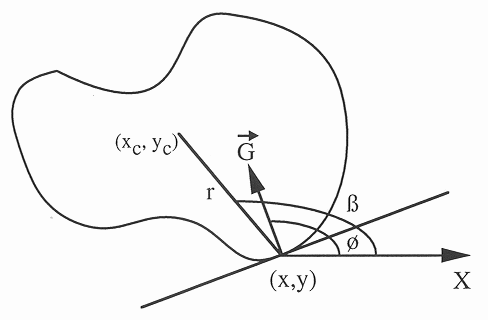
\includegraphics{shape_params}
    \label{fig:my_label}
\end{figure}

\column{.5\textwidth} % Right column and width
\begin{itemize}
    \item Usamos un punto de referencia $(x_c, y_c)$, por ejemplo el centroide
    \item Cada punto de borde tiene un vector $\textbf{r}$ asociado a su posición respecto de $(x_c, y_c)$. Podemos caracterizarlo con su módulo $r$ y ángulo $\beta$
    \item Sumamos la información direccional, esto es, el ángulo $\phi$ del vector gradiente
\end{itemize}
\end{columns}

\end{frame}
\subsection{La tabla-R}
\begin{frame}{La tabla R}
Con esta información podemos describir a la figura en la llamada \textit{tabla-$R$}
\begin{columns}[c] % The "c" option specifies centered vertical alignment while the "t" option is used for top vertical alignment

\column{.45\textwidth} % Left column and width
    \begin{figure}
    \centering
    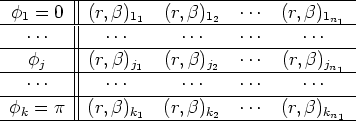
\includegraphics{rtable}
    \label{fig:my_label}
\end{figure}

\column{.5\textwidth} % Right column and width
\begin{itemize}
    \item La información de cada pixel de borde (esto es, los vectores \textbf{r}) se agrupa según la direccion del gradiente (se utiliza una discretización)
\end{itemize}
\end{columns}
\begin{itemize}
\item La tabla-R entonces es una descripción de la forma con información direccional
\item Transformaciones básicas de la tabla permiten expresar transformaciones de la forma
\end{itemize}

\end{frame}
\begin{frame}{Expresando transformaciones}
Notemos al conjunto de vectores de la tabla $R$ de una forma $\Gamma$ bajo la orientación $\phi$ por $R_\Gamma(\phi)$. ¿Cómo se transforma la tabla si se transforma la forma?
\begin{itemize}
    \item \textbf{Traslaciones}: la tabla no cambia, pues la información que tiene es relativa al centroide
    \item \textbf{Transformaciones de escala}: si $T_s$ es una transformación de escala donde la forma se ve escalada por $s$, entonces $R_{T_s(\Gamma)}(\phi) = sR_\Gamma(\phi)$, es decir, cada vector $\textbf{r}$ se ve escalado por $s$
    \item \textbf{Rotaciones}: si la forma se ve rotada por $\theta$ y llamamos a esa transformacion $T_\theta$, tenemos \[ R_{T_\theta(\Gamma)}(\phi) = Rot\{R_\Gamma[(\phi-\theta)\ mod\ 2\pi],\ \theta\} \]
    Esto es, tanto las orientaciones del gradiente como de los vectores \textbf{r} se ven modificadas.
\end{itemize}
\end{frame}
\begin{frame}{Construcción de la tabla-R}
    \begin{enumerate}
        \item Obtener la informacion de gradiente y los pixeles de borde para la imagen de referencia (el objeto o forma)
       \item Inicializar vacías las entradas de la tabla R para los ángulos $\phi_1, \phi_2, \cdots, \phi_n$ (siguiendo cierta discretización para $\phi$)
        \item Calcular un punto de referencia $(x_0, y_0)$ para la forma (por ejemplo el centroide)
        \item Para cada pixel de borde $(x,y)$, calcular:
            \[ 
                \begin{cases}
                    r = \sqrt{(x - x_0)^2 + (y-y_0)^2} \\
                    \beta = arctg (\frac{y_0 - y}{x_0 - x})
                \end{cases}
            \]
        \item Buscar $\phi_{x,y}$, la dirección del gradiente en ese pixel
        \item Guardar la entrada $(r, \beta)$ en $R(\phi_i)$, donde $\phi_i$ es el ángulo más cercano de la discretización a $\phi_{x,y}$
        \end{enumerate}
\end{frame}
\subsection{Algoritmo de detección}
\begin{frame}{Algoritmo de detección}
\begin{itemize}
    \item Construida la tabla-$R$, podemos detectar la forma en una imagen con transformaciones (como las descritas) arbitrarias
    \item El espacio de parámetros esta dado por $(x_0, y_0, s, \theta)$ 
    \item La información direccional nos permite reducir la búsqueda a entradas específicas de la tabla-$R$, y agrega precisión a la detección
    \item Los elementos de la tabla nos permiten determinar un centroide dados $s, \theta, x, y$ (similar a como se determinaba el centro de la elipse) 
\end{itemize}
\end{frame}
%------------------------------------------------
\begin{frame}{Algoritmo de detección}
    \begin{enumerate}
        \item Obtener la informacion de gradiente y los pixeles de borde para la imagen
        \item Inicializar en $0$ el vector de acumulación $A[x_0, y_0, s, \theta]$
        \item Para cada punto de borde (x,y), iterar por el subespacio de parámetros dado por $(s, \theta)$:
        \begin{itemize}
            \item Con la direción del gradiente $\phi_{x,y}$ obtener las entradas de la tabla-R en $R(\phi_{x,y} - \theta\ \mod 2\pi)$
            \item Para cada $(r, \beta)$ en esa entrada de la tabla determinar $x_0, y_0$ según:
                    \[ \begin{cases}
                      x_0 = x - s (r \cos (\beta + \theta))\\    
                      y_0 = y - s (r \sin (\beta + \theta))
                  \end{cases} \]
            \item Incrementar $A[x_0, y_0, s, \theta]$
        \end{itemize}
  \item Buscar máximos locales en $A$. Estos determinan los parámetros de la forma transformada en la imagen (posición del centroide, escala y rotación). 
    \end{enumerate}
    
\end{frame}
\begin{frame}{Ejemplo}
\begin{figure}
    \centering
    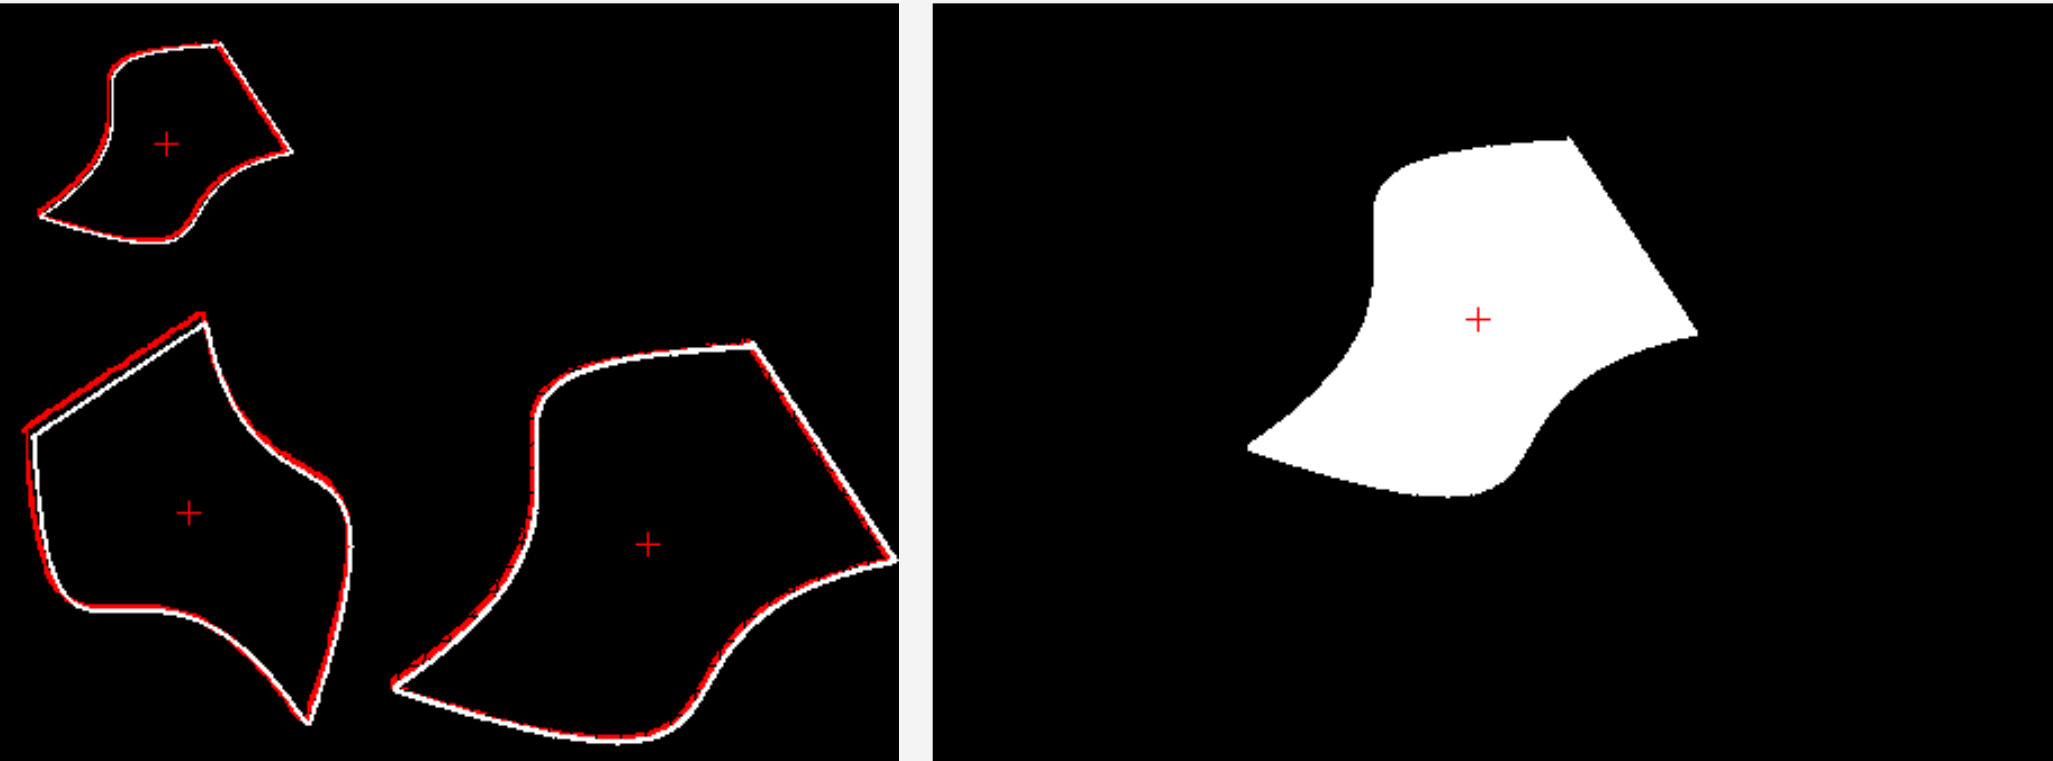
\includegraphics[scale=0.5]{ejemplo-sintetico}
    \label{fig:my_label}
\end{figure}
Detección con imágen sintética (se detecta la forma de la derecha en la imagen de la izquierda).
\end{frame}
\begin{frame}{Otros comentarios}
\begin{itemize}
    \item Podemos agregar más parámetros para expresar transformaciones
    \begin{itemize}
        \item en lugar de una escala uniforme $s$, dos parámetros de escala ortogonales ($s_x$, $s_y$)
        \item reflexiones
    \end{itemize}
    \item estas transformaciones afectan la determinación del centroide a la hora del voto (paso 3.2 del algoritmo anterior): en efecto son transformaciones de la tabla-R 
    \item El algoritmo es completamente paralelizable
\end{itemize}
\end{frame}

%\begin{frame}
%\Huge{\centerline{Fin}}
%\end{frame}

\end{document}